\documentclass[conference]{IEEEtran}

\IEEEoverridecommandlockouts
% The preceding line is only needed to identify funding in the first footnote. If that is unneeded, please comment it out.

% Packages
\usepackage{cite}
\usepackage{enumitem}
\usepackage{amsmath,amssymb,amsfonts}
\usepackage{algorithm}
\usepackage{algorithmic}
\usepackage{graphicx}
\usepackage{textcomp}
\usepackage{xcolor}
\usepackage{forest}
% \usetikzlibrary{trees,positioning,shapes,shadows,arrows.meta, calc}
\usepackage{tikz}
\usepackage{adjustbox} % For scaling the figure
\usepackage{url}

% Additional packages for figures and tables
\usepackage{pgfplots}
\usepackage{booktabs}  % For professional tables
\usepackage{colortbl}  % For colored table cells
% \usepackage{quantikz}  % For quantum circuits
% \pgfplotsset{compat=1.18}
\usetikzlibrary{shapes.geometric,arrows,positioning,fit,backgrounds,calc,decorations.pathreplacing,decorations.markings,patterns,circuits.logic.US,matrix,chains}

% Custom command for line breaks in author block
\makeatletter
\newcommand{\linebreakand}{%
  \end{@IEEEauthorhalign}
  \hfill\mbox{}\par
  \mbox{}\hfill\begin{@IEEEauthorhalign}
}
\makeatother

% Define quantum computing related colors
\definecolor{qubitblue}{RGB}{70,130,180}
\definecolor{controlred}{RGB}{220,20,60}
\definecolor{aigreen}{RGB}{50,150,50}
\definecolor{quantumpurple}{RGB}{128,0,128}
\definecolor{errororange}{RGB}{255,140,0}

\begin{document}

\title{Quantum Computing Enhanced by Artificial Intelligence: Principles and Applications}

\author{
    \IEEEauthorblockN{
        Benji Peng\textsuperscript{*, a, b},
        Chia Xin Liang \textsuperscript{c},
        Keyu Chen\textsuperscript{a},
        Ziqian Bi\textsuperscript{d}, 
        Ming Liu\textsuperscript{e},
        Yichao Zhang\textsuperscript{f}, \\
        Tianyang Wang\textsuperscript{g},
        Xinyuan Song \textsuperscript{h}
    }
    \IEEEauthorblockA{
        \textsuperscript{a}Georgia Institute of Technology, USA
    }
    \IEEEauthorblockA{
        \textsuperscript{b}AppCubic, USA
    }
    \IEEEauthorblockA{
        \textsuperscript{c}JTB Technology Corp., ROC
    }
    \IEEEauthorblockA{
        \textsuperscript{d}Indiana University, USA
    }
    \IEEEauthorblockA{
        \textsuperscript{e}Purdue University, USA
    }
    \IEEEauthorblockA{
        \textsuperscript{f}The University of Texas at Dallas, USA
    }
    \IEEEauthorblockA{
        \textsuperscript{g}University of Liverpool, UK
    }
    \IEEEauthorblockA{
        \textsuperscript{h}Emory University, USA
    }
    \IEEEauthorblockA{
        *Corresponding Email: benji@appcubic.com
    }
}

\maketitle

\begin{IEEEkeywords}
quantum computing, artificial intelligence, machine learning, neural networks, reinforcement learning, quantum error correction, quantum control
\end{IEEEkeywords}


\begin{abstract}
Artificial intelligence (AI) approaches are transforming quantum computing research across hardware, algorithms, and applications. The high-dimensional nature and unique properties of quantum systems align well with AI's pattern recognition capabilities. This article examines how modern AI techniques advance quantum computing development throughout the computing stack - from hardware design to execution and result interpretation. We explore the mathematical foundations, practical implementations, and emerging opportunities where AI can help overcome key technical barriers in quantum computing advancement.
\end{abstract}


\section{Introduction}
Quantum computing promises computational advantages for specific problems by harnessing quantum mechanical phenomena such as superposition and entanglement \cite{alexeev2021quantum}. As quantum hardware advances from noisy intermediate-scale quantum (NISQ) devices toward fault-tolerant systems, numerous technical challenges emerge across the quantum computing stack - from device physics to algorithm implementation.

Artificial intelligence offers powerful tools for addressing these challenges. The complex, high-dimensional, and non-linear nature of quantum systems makes them particularly amenable to AI approaches \cite{dunjko2023artificial}. Machine learning techniques excel at recognizing patterns in multidimensional spaces and optimizing complex functions - capabilities directly applicable to quantum computing problems.

This article explores applications of AI techniques for enhancing quantum computing development and operation. We focus on how AI accelerates quantum computing research and implementation rather than on quantum computing's potential future impact on AI itself. The content addresses the complete quantum computing workflow, from fundamental AI methods relevant to quantum applications through hardware optimization, circuit synthesis, control systems, error management, and error correction strategies. For each area, we present the mathematical foundations where appropriate and examine how AI techniques provide novel solutions to quantum computing challenges.

\begin{figure}[!t]
\centering
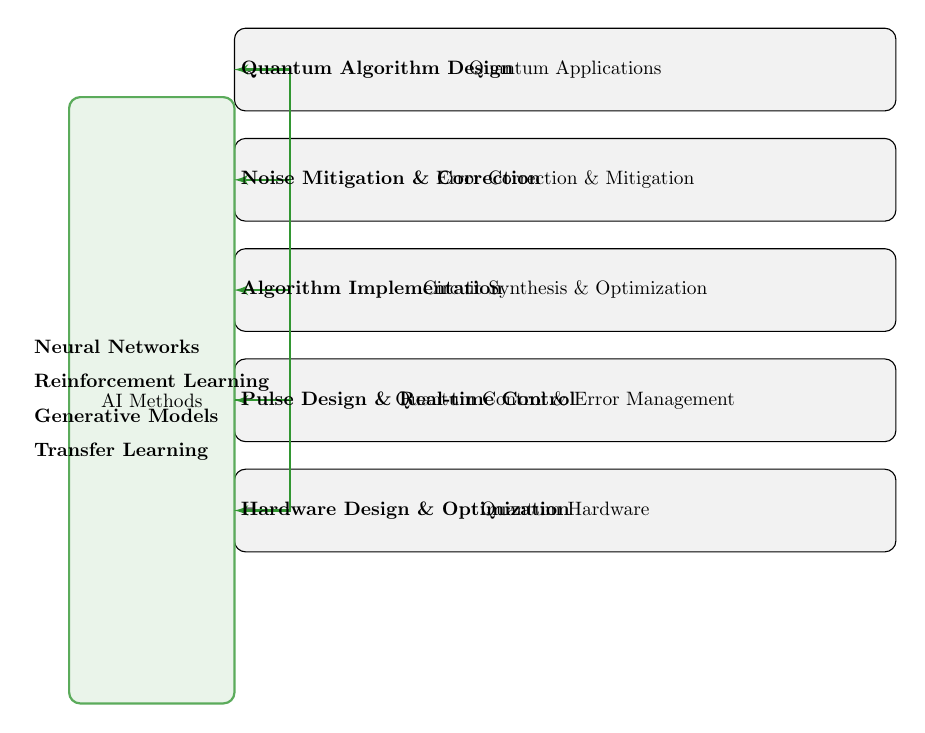
\begin{tikzpicture}[node distance=1.2cm, auto, >=latex', scale=0.7, transform shape]
    % Define nodes
    \node [rectangle, rounded corners, minimum width=12cm, minimum height=1.5cm, draw=black, fill=gray!10] (qh) {Quantum Hardware};
    \node [rectangle, rounded corners, minimum width=12cm, minimum height=1.5cm, draw=black, fill=gray!10, above of=qh, node distance=2cm] (ctl) {Quantum Control \& Error Management};
    \node [rectangle, rounded corners, minimum width=12cm, minimum height=1.5cm, draw=black, fill=gray!10, above of=ctl, node distance=2cm] (circ) {Circuit Synthesis \& Optimization};
    \node [rectangle, rounded corners, minimum width=12cm, minimum height=1.5cm, draw=black, fill=gray!10, above of=circ, node distance=2cm] (error) {Error Correction \& Mitigation};
    \node [rectangle, rounded corners, minimum width=12cm, minimum height=1.5cm, draw=black, fill=gray!10, above of=error, node distance=2cm] (app) {Quantum Applications};
    
    % Define AI box
    \node [rectangle, rounded corners, minimum width=3cm, minimum height=11cm, draw=aigreen!80, thick, fill=aigreen!10, left of=ctl, node distance=7.5cm] (ai) {AI Methods};
    
    % Define arrows
    \draw[->, thick, aigreen] (ai.east) -- ++(1,0) |- (qh.west);
    \draw[->, thick, aigreen] (ai.east) -- ++(1,0) |- (ctl.west);
    \draw[->, thick, aigreen] (ai.east) -- ++(1,0) |- (circ.west);
    \draw[->, thick, aigreen] (ai.east) -- ++(1,0) |- (error.west);
    \draw[->, thick, aigreen] (ai.east) -- ++(1,0) |- (app.west);
    
    % Labels for quantum computing layers
    \node[right] at (qh.west) {\textbf{Hardware Design \& Optimization}};
    \node[right] at (ctl.west) {\textbf{Pulse Design \& Real-time Control}};
    \node[right] at (circ.west) {\textbf{Algorithm Implementation}};
    \node[right] at (error.west) {\textbf{Noise Mitigation \& Correction}};
    \node[right] at (app.west) {\textbf{Quantum Algorithm Design}};
    
    % AI methods labels
    \node[align=left] at (ai) {
        \textbf{Neural Networks}\\[0.2cm]
        \textbf{Reinforcement Learning}\\[0.2cm]
        \textbf{Generative Models}\\[0.2cm]
        \textbf{Transfer Learning}
    };
    
\end{tikzpicture}
\caption{Integration of AI methods across the quantum computing stack. AI techniques enhance each layer of quantum computing development, from hardware design to application implementation. The bidirectional relationship enables advances in both fields, with quantum computing challenges driving AI innovation.}
\label{fig:ai_quantum_stack}
\end{figure}

\subsection{AI Paradigms for Quantum Computing}

Several key AI paradigms have demonstrated particular relevance to quantum computing challenges. Supervised learning models, trained on labeled data, can predict properties of quantum systems with remarkable accuracy. These methods have proven effective for tasks such as predicting the ground state energies of molecular systems or estimating the fidelity of quantum operations under noise.

Unsupervised learning techniques discover structure in quantum data without explicit labels. Such approaches have been successfully applied to identify patterns in experimental measurement results and to cluster quantum states according to their entanglement properties \cite{janiesch2021machine}.

Reinforcement learning (RL) has emerged as a particularly powerful paradigm for quantum computing \cite{arulkumaran2017deep, shakya2023reinforcement}. By formulating quantum control and optimization as sequential decision processes, RL agents learn optimal policies through direct interaction with quantum systems or their simulations. This approach has proven especially valuable for discovering non-intuitive control strategies that outperform conventional methods.

Deep learning architectures, with their ability to extract hierarchical features from complex data \cite{lecun2015deep}, provide the foundation for many quantum applications. These neural networks can process the high-dimensional data associated with quantum states and processes, enabling more efficient representation and manipulation of quantum information.

Generative models represent another crucial AI approach for quantum computing. These architectures create novel quantum circuits, control sequences, and error correction codes by learning probability distributions over complex quantum objects \cite{bernardo2007generative}. Recent advances in generative models have demonstrated their ability to discover quantum protocols that match or exceed those designed by human experts.

\subsection{Structure of this Article}

The remainder of this article is organized according to the quantum computing workflow. Section 2 examines fundamental AI techniques and their mathematical formulations relevant to quantum computing applications. Section 3 explores quantum hardware optimization, including system identification, device design, and pulse optimization. Section 4 addresses circuit synthesis and optimization, focusing on AI methods for transforming abstract algorithms into efficient implementations. Section 5 covers quantum control and error management during execution, while Section 6 explores AI approaches for error correction and mitigation. Finally, Sections 7 and 8 discuss emerging research directions and summarize the key insights regarding the synergy between AI and quantum computing. 

\section{AI Fundamentals for Quantum Computing}
AI techniques are particularly well-suited for quantum computing challenges due to their ability to handle high-dimensional data and complex optimization problems. This section examines the mathematical principles of key AI approaches and their quantum computing applications.

\subsection{Neural Networks for Quantum Systems}

Neural networks form the foundation of many AI approaches in quantum computing. A feed-forward neural network with $L$ layers can be expressed as a composition of functions:

\begin{equation}
f(x) = (f_L \circ f_{L-1} \circ \cdots \circ f_1)(x)
\end{equation}

where each layer $f_i(x) = \sigma(W_i x + b_i)$ applies a linear transformation followed by a non-linear activation function $\sigma$. The universal approximation theorem \cite{hornik1989multilayer} guarantees that such networks can represent arbitrarily complex functions - a critical property for modeling quantum phenomena.

\subsubsection{Architecture Specialization for Quantum Tasks}

Several neural network architectures have been specialized for quantum computing applications. Convolutional Neural Networks (CNNs) exploit spatial locality in quantum data, making them particularly effective for processing quantum state tomography results and error syndromes in topological codes. Their translation invariance properties align well with the spatial structure of many quantum error correction codes.

Recurrent Neural Networks (RNNs) excel at modeling temporal dynamics in quantum systems \cite{banchi2018modelling}. These architectures maintain an internal state that captures information about past inputs, enabling them to process sequence data such as quantum control pulses or time-dependent measurement records. Long Short-Term Memory (LSTM) networks and Gated Recurrent Units (GRUs) have proven especially effective for quantum control optimization tasks where temporal correlations span multiple timescales.

Graph Neural Networks (GNNs) process data structured as graphs, making them ideal for quantum circuits represented as directed acyclic graphs. In these applications, nodes represent quantum gates or operations, while edges represent qubit connections or information flow. GNNs have demonstrated significant advantages for circuit optimization and quantum architecture design by directly operating on the circuit's graph structure.

Transformer architectures, which leverage attention mechanisms to capture long-range dependencies, have recently been applied to quantum circuit design and control sequence optimization. These models can identify correlations between operations separated by significant circuit depth, enabling more efficient circuit synthesis and optimization.

\subsection{Reinforcement Learning for Quantum Control}

Reinforcement learning formulates quantum control as a Markov decision process (MDP), where states $s \in \mathcal{S}$ represent quantum system configurations, actions $a \in \mathcal{A}$ correspond to control operations, transition dynamics $P(s'|s,a)$ follow quantum mechanical laws, and reward function $R(s,a,s')$ measures control quality (e.g., gate fidelity).

RL aims to find a policy $\pi: \mathcal{S} \rightarrow \mathcal{A}$ maximizing expected cumulative reward:

\begin{equation}
J(\pi) = \mathbb{E}_{\tau \sim \pi}\left[\sum_{t=0}^{T} \gamma^t R(s_t, a_t, s_{t+1})\right]
\end{equation}

where $\tau$ represents a trajectory of states and actions, and $\gamma$ is a discount factor.

\subsubsection{RL Advantages for Quantum Applications}

For quantum control \cite{bukov2018reinforcement}, RL offers several significant advantages over traditional optimization approaches. First, RL enables exploration of non-intuitive control strategies beyond traditional approaches derived from analytical methods. This has led to the discovery of control protocols that achieve higher fidelities and shorter gate times than previously thought possible.

Second, RL methods demonstrate remarkable adaptability to quantum system variations and uncertainties. By incorporating system fluctuations into the training process, RL agents learn robust policies that maintain performance despite fabrication imperfections or environmental drift. This robustness is particularly valuable for real-world quantum hardware where ideal parameters are rarely achieved.

Third, RL provides end-to-end optimization without requiring analytical gradients of the objective function with respect to control parameters. This gradient-free approach is especially valuable for quantum systems where the exact relationship between controls and performance may be complex or unknown. Finally, RL algorithms can directly incorporate physical constraints into the learning process, ensuring that generated control sequences respect hardware limitations such as bandwidth constraints or maximum field strengths.

\subsection{Generative Models for Quantum States and Circuits}

Generative models learn probability distributions over quantum objects such as states, circuits, or control sequences. These models enable the creation of novel quantum protocols that may exceed human-designed approaches in efficiency or performance.

\subsubsection{Variational Autoencoders}

Variational Autoencoders (VAEs) provide a framework for learning compressed representations of quantum data. These models encode quantum states or circuits into a lower-dimensional latent space via an encoder network $q_\phi(z|x)$ and decode via $p_\theta(x|z)$, trained to maximize:

\begin{equation}
\mathcal{L}(\theta, \phi; x) = \mathbb{E}_{q_\phi(z|x)}[\log p_\theta(x|z)] - D_{KL}(q_\phi(z|x) || p(z))
\end{equation}

The first term encourages accurate reconstruction of input data, while the second term, the Kullback-Leibler divergence, ensures the latent space follows a prior distribution $p(z)$, typically a standard normal distribution. In quantum computing applications, VAEs have been used to discover efficient circuit representations and for quantum state compression.

\subsubsection{Adversarial and Diffusion Models}

Generative Adversarial Networks (GANs) employ a competitive training process between a generator $G(z)$ and discriminator $D(x)$. The generator creates quantum circuits or states from random noise, while the discriminator attempts to distinguish these generated samples from real examples. Through this adversarial process, the generator learns to produce increasingly realistic quantum objects. GANs have been applied to generate quantum circuits for specific tasks and to create synthetic quantum data for training other machine learning models.

Diffusion models represent a more recent approach to quantum circuit generation \cite{furrutter2024quantum}. These models work by learning to reverse a gradual noising process, starting from a complex circuit and progressively simplifying it through noise addition. By inverting this process, diffusion models can generate high-quality quantum circuits starting from random noise. Recent work has demonstrated that diffusion models can discover circuit implementations that match or exceed those designed by human experts, particularly for complex unitary operations.

\subsection{Transfer Learning for Quantum Tasks}

Transfer learning addresses the challenge of limited training data in quantum computing by adapting models trained on one quantum task to another related task. For a source task $\mathcal{T}_S$ and target task $\mathcal{T}_T$, knowledge transfer occurs when:

\begin{equation}
P(Y_T | X_T) = \int P(Y_T | X_T, K) P(K | \mathcal{T}_S) dK
\end{equation}

where $K$ represents transferable knowledge.

This approach has proven valuable for transferring learned representations between similar quantum hardware platforms. For example, models trained on simulated quantum devices can be fine-tuned with limited data from real hardware, significantly accelerating the development of hardware-specific control strategies. Similarly, control policies learned on smaller quantum systems can be transferred to larger systems, helping address the exponential scaling challenge of quantum simulation.

Transfer learning has also demonstrated success in adapting error correction decoders to larger code distances. By training on smaller, tractable codes and transferring knowledge to larger codes, researchers have developed decoders that scale more efficiently than those trained from scratch on each code size. This scalability is crucial for practical quantum error correction, where code distances must increase as quantum computers grow in size.

These mathematical frameworks provide powerful tools for addressing quantum computing challenges, with implementations demonstrating clear advantages over traditional methods across multiple domains of the quantum computing stack. 

\section{Quantum Hardware Optimization}
This section examines how AI techniques are being applied to quantum hardware design, characterization, and optimization.

\subsection{System Characterization}
AI methods are increasingly employed to characterize quantum systems, addressing challenges in Hamiltonian learning \cite{wiebe2014hamiltonian, gentile2021learning} and noise modeling. Machine learning approaches can extract valuable information about system parameters and environmental interactions from experimental data, often outperforming traditional characterization methods.

\subsection{Platform Design}
The design of quantum computing platforms involves complex optimization challenges across multiple physical layers. AI techniques are helping researchers navigate these design spaces more efficiently, from materials selection to device layout and architecture.

\subsection{Gate and Pulse Optimization}
Quantum gate implementation through optimized control pulses is a critical area where AI has demonstrated significant advantages. Reinforcement learning approaches have proven particularly effective for discovering high-fidelity control pulses \cite{bukov2018reinforcement, ding2021breaking}. 

\section{Circuit Synthesis and Optimization}
Before executing quantum algorithms, several preprocessing steps can significantly impact performance. This section explores how AI is enhancing these preparatory phases.

\subsection{Quantum Circuit Synthesis}
Converting algorithms to efficient quantum circuits presents numerous challenges that AI methods are helping to address.

\subsubsection{Unitary Synthesis}
AI techniques are providing new approaches to decomposing arbitrary unitary operations into sequences of available gates, often finding more efficient implementations than traditional decomposition methods.

\subsubsection{AI Models to Generate Compact Circuits}
Recent work with generative models has shown promise in creating more compact circuit representations, potentially reducing resource requirements for quantum algorithms.

\subsection{Circuit Parameter Learning and Parameter Transfer}
For parameterized quantum circuits, finding optimal parameters is challenging due to issues like barren plateaus. AI methods can help navigate these complex optimization landscapes more effectively.

\subsection{State Preparation}
Preparing specific quantum states efficiently is crucial for many algorithms. AI approaches are helping develop improved state preparation protocols that require fewer operations and are more robust to noise. 

\section{Quantum Control and Error Management}
Controlling quantum systems with high fidelity presents unique challenges that AI methods are particularly well-suited to address. This section examines how AI is improving quantum device control and optimization.

Reinforcement learning has emerged as a powerful approach for quantum control optimization, allowing the discovery of control sequences that outperform those designed using conventional methods. Key applications include:

\begin{itemize}
    \item Optimizing single and multi-qubit gate implementations
    \item Developing robust control sequences that maintain performance despite system variations
    \item Real-time adaptive control based on measurement feedback
    \item Learning control strategies for complex many-body quantum systems
\end{itemize}

Recent work has demonstrated how reinforcement learning agents can break constraints imposed by adiabatic quantum control \cite{ding2021breaking}, potentially opening new routes to high-fidelity quantum operations. 

Quantum systems require precise control to maintain coherence and execute operations with high fidelity. AI techniques offer significant advantages for both offline control optimization and real-time error management.

\subsection{Optimal Control Theory}
Quantum optimal control seeks time-dependent control fields $\{c_j(t)\}$ that drive a quantum system governed by the Hamiltonian:

\begin{equation}
H(t) = H_0 + \sum_j c_j(t) H_j
\end{equation}

where $H_0$ is the drift Hamiltonian and $\{H_j\}$ are control Hamiltonians. The goal is to evolve the system from an initial state $\rho_0$ to a target state $\rho_T$ or to implement a target unitary $U_T$.

Traditional approaches like GRAPE (Gradient Ascent Pulse Engineering) use gradient information to optimize control parameters. AI methods extend these capabilities through:

\begin{itemize}
    \item \textbf{Model-free optimization}: Reinforcement learning agents can discover high-fidelity control sequences without explicit system models \cite{bukov2018reinforcement}
    
    \item \textbf{Robustness to uncertainty}: Neural network controllers can maintain performance despite variations in system parameters
    
    \item \textbf{Breaking adiabatic constraints}: RL approaches have discovered control protocols that exceed the speed limits of adiabatic control \cite{ding2021breaking}
\end{itemize}

\subsection{Real-time Adaptive Control}
Real-time control adjusts operations based on continuous measurement feedback. For a partially observable quantum system, the control problem becomes a partially observable Markov decision process (POMDP) where:

\begin{itemize}
    \item States represent quantum density matrices $\rho$
    \item Actions are control operations
    \item Observations are measurement outcomes with probability distributions determined by quantum mechanics
\end{itemize}

Deep reinforcement learning strategies for this POMDP can be formulated using recurrent neural networks that maintain internal representations of quantum state estimates. The resulting controllers can:

\begin{equation}
\pi(a_t | o_1, o_2, \ldots, o_t) = \text{RNN}(o_t, h_{t-1})
\end{equation}

where $o_t$ are observations, $a_t$ are actions, and $h_t$ is the hidden state of the RNN.

\subsection{Multi-qubit Operation Scheduling}
Executing multiple operations across a quantum processor requires sophisticated scheduling to minimize crosstalk and maximize parallelism. Machine learning approaches formulate this as a constrained optimization problem:

\begin{equation}
\min_{\{t_i\}} \sum_i w_i t_i \quad \text{subject to constraints on overlapping operations}
\end{equation}

where $t_i$ represents the start time of operation $i$ and $w_i$ its priority weight.

AI schedulers can consider hardware-specific constraints such as:
\begin{itemize}
    \item Control line bandwidth limitations
    \item Crosstalk between neighboring qubits
    \item Time-dependent noise characteristics
    \item Variability in operation fidelities
\end{itemize}

\subsection{In-situ Calibration and Drift Compensation}
Quantum systems exhibit parameter drift over time, requiring continuous recalibration. AI techniques enable efficient in-situ calibration through:

\begin{itemize}
    \item \textbf{Bayesian experimental design}: Selecting optimal calibration experiments to maximize information gain
    
    \item \textbf{Online learning}: Continuously updating system models based on observed performance
    
    \item \textbf{Predictive maintenance}: Forecasting parameter drift and scheduling preventive recalibration
\end{itemize}

These control techniques significantly enhance quantum computer performance by optimizing hardware operation at multiple timescales - from nanosecond pulse shaping to millisecond measurement feedback and hour-to-hour drift compensation. 

\section{Error Correction and Mitigation}
Error management is essential for reliable quantum computation. This section examines AI approaches for both error correction and mitigation.

\subsection{Neural Decoders for Quantum Error Correction}

Quantum error correction (QEC) detects and corrects errors through syndrome measurements. For a stabilizer code with stabilizer group $\mathcal{S}$, the decoding problem involves:

\begin{enumerate}
    \item Measuring syndrome bits $s_i = \langle \psi | S_i | \psi \rangle$ for stabilizers $S_i \in \mathcal{S}$
    \item Inferring the most likely error $E$ given syndrome pattern $s$: $P(E|s)$
    \item Applying the appropriate recovery operation $R$
\end{enumerate}

Traditional decoding approaches include minimum-weight perfect matching for surface codes and belief propagation for LDPC codes. While these methods provide theoretical guarantees, they often struggle with realistic noise models and hardware constraints. Neural network decoders address these limitations by framing decoding as a classification problem, mapping syndromes to recovery operations:

\begin{equation}
f_\theta: \{0,1\}^m \rightarrow \mathcal{P}^n
\end{equation}

where $m$ is the number of syndrome bits, $n$ is the number of physical qubits, and $\mathcal{P}^n$ is the Pauli group on $n$ qubits.

\subsubsection{Speed and Latency Advantages}

Neural decoders achieve microsecond-scale decoding latency, critical for real-time error correction. This speed advantage stems from their feed-forward architecture, which requires only matrix multiplications and simple non-linear operations after training. Traditional decoders often require iterative graph-based algorithms with unpredictable convergence times. Recent implementations using field-programmable gate arrays (FPGAs) have demonstrated neural decoders operating within the coherence time constraints of superconducting qubit systems, enabling real-time feed-forward correction \cite{ryan2021realization}.

\subsubsection{Noise-Adaptive Decoding}

A key advantage of machine learning decoders is their adaptability to device-specific noise profiles. While traditional decoders typically assume idealized noise models such as independent depolarizing noise, neural network decoders can be trained directly on the noise characteristics of specific hardware. This training can incorporate spatially and temporally correlated errors, coherent error mechanisms, and measurement imperfections.

Convolutional neural networks have proven particularly effective for decoding topological codes like the surface code, where error correlations exhibit spatial locality. The translation invariance properties of CNNs align well with the regular lattice structure of these codes, enabling efficient parameter sharing. For codes without spatial structure, transformer architectures have demonstrated promising results by capturing long-range dependencies between syndrome bits.

\subsubsection{Scalability to Larger Codes}

Traditional decoding algorithms often face challenges scaling to larger code distances due to increasing computational complexity. Architecture designs like convolutional decoders scale efficiently to larger code distances because they leverage parameter sharing across the code lattice. Transfer learning techniques further enhance scalability by training decoders on smaller codes and transferring knowledge to larger codes, significantly reducing the training data requirements for large-scale error correction.

Recent implementations have demonstrated neural decoders with performance approaching or exceeding traditional algorithms like minimum-weight perfect matching, but with significantly reduced computational overhead. These advantages become particularly pronounced for complex noise models and when decoding must be performed under strict time constraints.

\begin{figure}[!t]
\centering
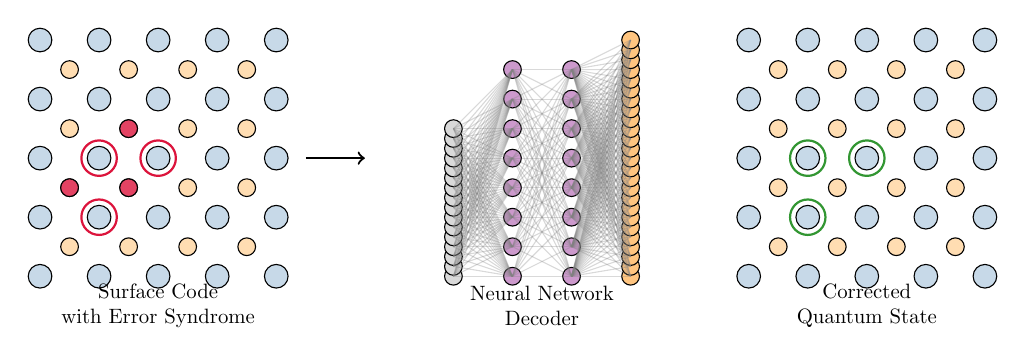
\begin{tikzpicture}[scale=0.75, transform shape]
    % Surface code lattice
    \begin{scope}[shift={(0,0)}]
        % Data qubits
        \foreach \i in {0,1,2,3,4} {
            \foreach \j in {0,1,2,3,4} {
                \filldraw[fill=qubitblue!30] (\i,\j) circle (0.2);
            }
        }
        
        % X-stabilizers (plaquettes)
        \foreach \i in {0.5,1.5,2.5,3.5} {
            \foreach \j in {0.5,1.5,2.5,3.5} {
                \filldraw[fill=errororange!30] (\i,\j) circle (0.15);
            }
        }
        
        % Error on some qubits
        \draw[thick, controlred] (1,1) circle (0.3);
        \draw[thick, controlred] (2,2) circle (0.3);
        \draw[thick, controlred] (1,2) circle (0.3);
        
        % Syndrome measurements (detected errors)
        \filldraw[fill=controlred!80] (1.5,1.5) circle (0.15);
        \filldraw[fill=controlred!80] (0.5,1.5) circle (0.15);
        \filldraw[fill=controlred!80] (1.5,2.5) circle (0.15);
        
        \node[align=center] at (2,-0.5) {Surface Code\\with Error Syndrome};
    \end{scope}
    
    % Neural network decoder
    \begin{scope}[shift={(7,0)}]
        % Input layer - syndrome
        \foreach \i in {0,...,3} {
            \foreach \j in {0,...,3} {
                \filldraw[fill=gray!30] (0,\i/1.5+\j/6) circle (0.15);
            }
        }
        
        % Hidden layers
        \foreach \i in {0,...,7} {
            \filldraw[fill=quantumpurple!40] (1,\i/2) circle (0.15);
        }
        
        \foreach \i in {0,...,7} {
            \filldraw[fill=quantumpurple!40] (2,\i/2) circle (0.15);
        }
        
        % Output layer - correction
        \foreach \i in {0,...,4} {
            \foreach \j in {0,...,4} {
                \filldraw[fill=errororange!50] (3,\i/1.2+\j/6) circle (0.15);
            }
        }
        
        % Connect layers
        \foreach \i in {0,...,3} {
            \foreach \j in {0,...,3} {
                \foreach \k in {0,...,7} {
                    \draw[gray, thin, opacity=0.3] (0,\i/1.5+\j/6) -- (1,\k/2);
                }
            }
        }
        
        \foreach \i in {0,...,7} {
            \foreach \j in {0,...,7} {
                \draw[gray, thin, opacity=0.3] (1,\i/2) -- (2,\j/2);
            }
        }
        
        \foreach \i in {0,...,7} {
            \foreach \j in {0,...,4} {
                \foreach \k in {0,...,4} {
                    \draw[gray, thin, opacity=0.3] (2,\i/2) -- (3,\j/1.2+\k/6);
                }
            }
        }
        
        \node[align=center] at (1.5,-0.5) {Neural Network\\Decoder};
    \end{scope}
    
    % Arrow connecting them
    \draw[->, thick] (4.5,2) -- (5.5,2);
    
    % Recovered state with correction
    \begin{scope}[shift={(12,0)}]
        % Data qubits
        \foreach \i in {0,1,2,3,4} {
            \foreach \j in {0,1,2,3,4} {
                \filldraw[fill=qubitblue!30] (\i,\j) circle (0.2);
            }
        }
        
        % X-stabilizers (plaquettes)
        \foreach \i in {0.5,1.5,2.5,3.5} {
            \foreach \j in {0.5,1.5,2.5,3.5} {
                \filldraw[fill=errororange!30] (\i,\j) circle (0.15);
            }
        }
        
        % Correction operations
        \draw[thick, aigreen] (1,1) circle (0.3);
        \draw[thick, aigreen] (2,2) circle (0.3);
        \draw[thick, aigreen] (1,2) circle (0.3);
        
        \node[align=center] at (2,-0.5) {Corrected\\Quantum State};
    \end{scope}
\end{tikzpicture}
\caption{Neural network-based decoding for the surface code. Left: A surface code lattice with data qubits (blue circles) and stabilizer measurements (orange circles). Errors on data qubits (red circles) cause syndrome measurements to detect stabilizer violations (red plaquettes). Center: A neural network processes the syndrome pattern to predict the most likely error configuration. Right: The decoder output determines correction operations (green circles) that restore the encoded quantum information.}
\label{fig:neural_decoder}
\end{figure}

\subsection{Error Correction Code Discovery}

The search for optimal quantum error correction codes presents a complex discrete optimization problem. Traditional code constructions rely on mathematical insights and specific algebraic structures, limiting exploration of the full code space. AI methods overcome these limitations by systematically exploring broader classes of codes.

\subsubsection{Reinforcement Learning for Code Construction}

Reinforcement learning agents can iteratively construct stabilizer sets, receiving rewards based on code distance and rate. The RL agent selects stabilizer generators sequentially, evaluating the resulting code properties after each selection. This approach allows exploration of non-standard code structures that might be overlooked by analytical methods. For example, RL-based searches have discovered surface codes with improved thresholds for biased noise models, outperforming standard constructions optimized for depolarizing noise.

\subsubsection{Genetic Algorithms and Evolutionary Approaches}

Evolutionary approaches "breed" promising codes to discover improved variants. Starting with a population of candidate codes, genetic algorithms apply mutation and crossover operations to generate new codes. Selection criteria based on code distance, encoding rate, and threshold under realistic noise preserve the most promising candidates for further evolution. This technique has proven particularly effective for tailoring codes to specific hardware constraints and noise models.

\subsubsection{Neural Architecture Approaches}

Autoencoder architectures represent another promising direction for code discovery. Neural networks can be trained to discover efficient encodings into protected subspaces by learning to reconstruct input states after passing through noisy channels. These learned encodings sometimes correspond to known quantum error correction codes but can also discover novel protection strategies. Recent work has shown that autoencoders can identify decoherence-free subspaces and noiseless subsystems for specific environmental coupling models.

These AI-based approaches have discovered codes with improved distance properties and efficient encoding/decoding circuits tailored to specific hardware constraints. By optimizing codes for the particular characteristics of available quantum hardware rather than idealized noise models, these techniques enable more effective error correction with limited resources.

\subsection{Error Mitigation Techniques}

For near-term quantum devices without full error correction, error mitigation techniques improve computational results. Unlike quantum error correction, which requires significant qubit overhead, error mitigation operates directly on noisy results with classical post-processing. AI methods have enhanced several key mitigation approaches.

\subsubsection{Zero-Noise Extrapolation}

Zero-noise extrapolation estimates error-free results by measuring observables at different artificial noise levels and extrapolating to the zero-noise limit. Machine learning models improve this extrapolation, predicting zero-noise limits from measurements at different noise levels:

\begin{equation}
\langle O \rangle_{\text{ideal}} \approx f_\theta(\langle O \rangle_{\lambda_1}, \langle O \rangle_{\lambda_2}, \ldots, \langle O \rangle_{\lambda_k})
\end{equation}

where $\langle O \rangle_{\lambda_i}$ represents expectation values at noise scale $\lambda_i$. Neural networks trained on simulated data learn to recognize the functional form of noise scaling for specific circuits and observables, enabling more accurate extrapolation than simple polynomial fits. These models also identify optimal noise scaling points to measure, reducing the number of circuit evaluations required.

\subsubsection{Quantum Subspace Expansion}

Quantum subspace expansion mitigates errors by projecting noisy results onto a smaller subspace that preserves relevant problem structure. Neural networks can identify optimal subspaces that minimize error effects by analyzing the structure of both the problem Hamiltonian and the device noise model. For electronic structure calculations, machine learning approaches have identified symmetry-preserving subspaces that significantly improve energy estimation accuracy even in the presence of substantial device noise.

\subsubsection{Measurement Error Mitigation}

Readout errors represent a significant source of computational inaccuracy in current quantum devices. Machine learning models learn calibration matrices that correct for readout errors:

\begin{equation}
\vec{p}_{\text{true}} = A^{-1} \vec{p}_{\text{measured}}
\end{equation}

where $A$ is the calibration matrix and $\vec{p}$ represents measurement outcome probabilities. Neural networks can model complex readout error patterns, including state-dependent errors and temporal correlations that simple calibration matrices cannot capture. By incorporating these detailed error models, ML-enhanced readout error mitigation significantly improves measurement accuracy for multi-qubit systems.

\subsubsection{Adaptive Measurement and Tomography}

AI techniques enable more efficient quantum state characterization through adaptive measurement strategies. Traditional approaches to quantum state tomography require exponentially many measurements with qubit count, making full characterization infeasible for even moderate-sized systems.

\subsubsection{Bayesian Experimental Design}

Bayesian experimental design selects optimal measurements to maximize information gain about quantum states. This approach maintains a probability distribution over possible quantum states and selects measurements that most effectively reduce uncertainty. Neural networks accelerate this process by predicting information gain for potential measurements without requiring expensive Monte Carlo sampling, enabling real-time adaptive measurement selection. These techniques have demonstrated order-of-magnitude reductions in the number of measurements required for state tomography compared to non-adaptive protocols.

\subsubsection{Compressed Sensing Approaches}

Compressed sensing reconstructs quantum states from an incomplete set of measurements by exploiting state sparsity in appropriate bases. This approach can be formulated as:

\begin{equation}
\min_\rho \|\rho\|_1 \quad \text{subject to} \quad \|y - \mathcal{A}(\rho)\|_2 < \epsilon
\end{equation}

where $y$ represents measurement outcomes, $\mathcal{A}$ is the measurement operator, and $\rho$ is the density matrix. Machine learning enhances compressed sensing by learning effective sparsifying transformations from data and accelerating the reconstruction optimization. These improvements enable accurate reconstruction of quantum states with substantially fewer measurements than required by traditional tomography protocols.

\subsubsection{Direct State Reconstruction}

Neural tomography networks directly map measurement statistics to density matrix estimates, bypassing iterative reconstruction algorithms. These networks learn to recognize patterns in measurement data that indicate specific quantum state features, enabling rapid reconstruction with limited data. Convolutional architectures have proven particularly effective for reconstructing states with local correlations, such as those appearing in many condensed matter systems and quantum simulation experiments.

The integration of these error correction and mitigation techniques, enhanced by AI, enables more reliable computation on both current and future quantum hardware. By tailoring error management strategies to specific devices and computational tasks, these approaches maximize the utility of available quantum resources.

\begin{table}[!t]
\centering
\caption{Comparison of AI-Enhanced Error Mitigation Techniques}
\label{tab:error_mitigation}
\scalebox{0.9}{
\begin{tabular}{@{}p{3cm}p{4cm}p{2.5cm}p{2.5cm}@{}}
\toprule
\textbf{Technique} & \textbf{AI Enhancement} & \textbf{Accuracy Improvement} & \textbf{Computational Overhead} \\
\midrule
Zero-Noise Extrapolation & Neural network for non-linear extrapolation & 2-5× reduction in error & Moderate (multiple circuit runs) \\
\midrule
Quantum Subspace Expansion & ML-identified optimal subspaces & 3-10× reduction in error & High (many additional measurements) \\
\midrule
Measurement Error Mitigation & NN-based correction beyond linear calibration & 5-20× reduction in readout error & Low (post-processing only) \\
\midrule
Adaptive Measurement & Bayesian experimental design with NNs & 2-4× reduction in tomography error & Moderate (real-time processing) \\
\bottomrule
\end{tabular}}
\end{table} 
% The content of this file has been integrated into the error_correction.tex file
% This file is retained for backward compatibility but is no longer used directly

After quantum computation, various postprocessing techniques can enhance the value of measurement results. This section examines how AI is improving these final stages of the quantum computing workflow.

\subsection{Efficient Observable Estimation and Tomography}
AI methods are enhancing our ability to extract information from limited measurement data, a crucial capability given the cost of quantum computation.

\subsection{Readout Measurements}
Accurate interpretation of measurement results in the presence of readout errors is essential. AI techniques are providing improved methods for:

\begin{itemize}
    \item Readout error mitigation
    \item Discrimination between quantum states
    \item Optimizing measurement procedures
\end{itemize}

\subsection{Error Mitigation Techniques}
Various error mitigation techniques can improve the quality of results from noisy quantum computers. AI methods are enhancing these approaches through:

\begin{itemize}
    \item Learning optimal error extrapolation strategies
    \item Identifying efficient noise-aware circuit transformations
    \item Developing hardware-adaptive error mitigation protocols
\end{itemize} 

\section{Future Directions}
The intersection of AI and quantum computing continues to evolve rapidly. This section highlights emerging research directions and technical challenges that will shape future developments.

\subsection{Foundation Models for Quantum Computing}

Large-scale foundation models that capture extensive knowledge about quantum systems represent a promising direction for future research. These models, inspired by the success of foundation models in natural language processing and computer vision, would encode broad knowledge about quantum systems and algorithms that could be fine-tuned for specific applications.

Foundation models could revolutionize quantum algorithm design by synthesizing quantum circuits based on high-level specifications. Rather than requiring detailed circuit construction, researchers could describe desired functionality in abstract terms, with the model generating appropriate implementations. This capability would significantly accelerate algorithm development and make quantum computing more accessible to domain experts without detailed quantum programming knowledge.

Another valuable application would be predicting quantum system behaviors across diverse physical platforms. By training on simulation data and experimental results from multiple quantum computing modalities, these models could transfer insights between different physical implementations. This cross-platform knowledge transfer would help identify common principles and best practices across quantum computing technologies.

Natural language interfaces for quantum algorithm design represent another promising direction. By understanding the semantic content of problem descriptions, foundation models could bridge the gap between problem specification and quantum implementation. Recent work in code generation from natural language specifications demonstrates the potential of this approach, which could be extended to the quantum domain.

The development of these foundation models will require significant advances in both training methodologies and quantum-specific architectures. Current approaches like transformers may need adaptation to better capture the unique structures of quantum data, such as the complex-valued nature of quantum states and the hierarchical organization of quantum circuits.

\subsection{Differentiable Quantum Programming}

End-to-end differentiable quantum programming environments will enable seamless integration of classical and quantum optimization. These environments allow gradients to flow through the entire quantum-classical computational pipeline, enabling more efficient optimization of hybrid quantum-classical algorithms.

Differentiable quantum simulators represent a key component of this approach. By implementing quantum operations in a manner that supports automatic differentiation, these simulators enable gradient-based optimization of entire quantum workflows. Current implementations like Pennylane and TensorFlow Quantum demonstrate the potential of this approach, though challenges remain in scaling to larger quantum systems and incorporating realistic noise models.

Automatic differentiation systems that handle the complexities of quantum operations present another research direction. Quantum operations involve complex numbers, unitary constraints, and measurement-induced non-linearities that require specialized differentiation rules. Developing efficient automatic differentiation techniques for these operations will accelerate the optimization of quantum algorithms and control sequences.

Hardware-aware gradient computation that accounts for device-specific noise characteristics represents a particularly valuable capability. By incorporating noise models into the differentiation process, these systems could optimize algorithms for specific quantum hardware rather than idealized models. This noise-aware optimization would produce circuits better suited for near-term quantum devices with significant error rates.

These advances will accelerate the co-design of quantum algorithms and hardware by enabling rapid exploration of design spaces. Rather than treating hardware capabilities as fixed constraints, differentiable programming environments would allow simultaneous optimization of algorithm structure and hardware parameters, potentially identifying synergistic configurations that would be missed by separate optimization processes.

\subsection{Active Learning for Quantum Experimentation}

Efficient exploration of quantum phenomena requires intelligent experimental design. As quantum systems grow in complexity, the space of possible experiments expands exponentially, making exhaustive exploration infeasible. Active learning approaches that optimize experiment selection will become increasingly important for characterizing quantum devices and discovering novel quantum phenomena.

Bayesian optimization frameworks provide principled approaches for quantum experiment design. By modeling the information gain of potential experiments, these frameworks select measurements that maximally reduce uncertainty about system parameters or behaviors. This approach has already demonstrated value for tasks like Hamiltonian learning and device calibration, where it significantly reduces the number of experiments required.

Reinforcement learning agents that adaptively control experimental parameters offer another promising direction. These agents can optimize complex experimental sequences with many control parameters, learning from the results of previous experiments to improve future performance. RL approaches are particularly valuable when the relationship between control parameters and experimental outcomes is complex or poorly understood.

Uncertainty-aware models that identify critical knowledge gaps provide another tool for efficient experimental design. By explicitly modeling uncertainty in system understanding, these approaches can direct experimental resources toward the most uncertain aspects of the system. This targeted exploration accelerates scientific discovery by focusing on regions of parameter space with the greatest potential for new insights.

These techniques will accelerate the characterization of quantum devices and the exploration of novel quantum phenomena. By replacing manual trial-and-error approaches with principled, automated experimental design, they will enable more efficient utilization of limited experimental resources and accelerate progress in quantum hardware development.

\subsection{Hardware-Software Co-optimization}

The tight coupling between quantum hardware and software necessitates co-optimization approaches that consider both aspects simultaneously. Traditional approaches that optimize hardware and software separately often miss opportunities for synergistic improvements that arise from their interdependence.

AI-driven compilation frameworks that adapt quantum programs to specific hardware capabilities represent an important step toward co-optimization. These frameworks analyze both algorithm structure and hardware characteristics to identify optimal implementations. For example, reinforcement learning-based compilers can discover qubit mapping strategies that minimize communication overhead on specific device topologies, significantly reducing circuit depth and improving computational fidelity.

Dynamic resource allocation systems will optimize quantum-classical computational boundaries based on the specific requirements of each algorithm component. By analyzing which portions of a computation benefit most from quantum processing and which are better handled classically, these systems can allocate computational resources more efficiently. This adaptive allocation maximizes the utility of limited quantum resources while leveraging classical computing capabilities where appropriate.

Automated design space exploration across both hardware and algorithm parameters will identify optimal configurations that might be missed by separate optimization processes. Machine learning models can efficiently navigate the combined hardware-software design space, identifying non-obvious parameter combinations that yield superior performance. This holistic optimization approach will become increasingly important as quantum systems grow in complexity and the design space expands.

\subsection{Technical Challenges}

Several technical challenges must be addressed to fully realize the potential of AI in quantum computing.

\subsubsection{Training Data Limitations}

Generating representative training data for quantum systems remains difficult, particularly for large-scale quantum systems that cannot be efficiently simulated classically. This challenge creates a circular dependency: AI models are needed to optimize large quantum systems, but training these models requires data from such systems. Several approaches may help address this challenge.

Transfer learning from smaller, simulable systems to larger ones offers one potential solution. By identifying patterns and principles that generalize across system sizes, models trained on small systems can provide useful initializations for larger systems. This approach has shown promise for tasks like error correction decoding and circuit optimization.

Hybrid data generation strategies that combine limited experimental data with simulation results represent another promising direction. By calibrating simulations based on experimental measurements from real quantum hardware, researchers can generate more realistic training data than would be possible from either source alone. This approach has been successfully applied to pulse optimization and readout error correction.

Unsupervised and self-supervised learning methods that require less labeled data may also help address data limitations. These approaches learn useful representations from unlabeled data, which is often more abundant than labeled examples. Recent advances in contrastive learning and generative modeling suggest potential applications to quantum data.

\subsubsection{Model Interpretability}

Understanding why AI models make specific decisions is crucial for scientific applications but remains challenging. Black-box models risk missing important physical insights and may make unreliable predictions when faced with situations outside their training distribution.

Physics-informed neural networks that incorporate known physical principles into model architecture represent one approach to improving interpretability. By constraining models to respect physical laws like unitarity or energy conservation, these networks produce more interpretable and reliable results. This approach has shown promise for tasks like Hamiltonian learning and quantum state tomography.

Attention mechanisms that highlight which input features most strongly influence model decisions provide another tool for interpretation. By examining attention weights, researchers can identify which system components or parameters drive particular behaviors. This insight can guide further investigation and hypothesis formation about underlying physical mechanisms.

Symbolic regression techniques that extract analytical expressions from trained models offer perhaps the most direct path to interpretability. These methods distill neural network knowledge into explicit mathematical formulas that can be analyzed and understood by humans. Recent advances in automated scientific discovery suggest potential applications to quantum control and algorithm design.

\subsubsection{Hardware Resource Constraints}

Real-time AI for quantum control requires models that can execute within strict timing constraints on specialized control hardware. Many current AI approaches involve computational requirements incompatible with the microsecond-scale feedback needed for quantum error correction and adaptive control.

Model compression techniques that reduce neural network size while preserving performance will be essential for deployment on control hardware. Approaches like pruning, quantization, and knowledge distillation can significantly reduce model size and computational requirements without substantial performance degradation. These techniques have already enabled neural decoders to operate within the coherence time constraints of superconducting qubit systems.

Hardware-specific model optimization that accounts for the capabilities and limitations of control electronics represents another important direction. By designing models specifically for the target hardware platform—whether FPGAs, ASICs, or other specialized processors—researchers can maximize performance within resource constraints. This co-design of models and hardware will be crucial for real-time quantum control applications.

Addressing these challenges will require continued collaboration between quantum physics, computer science, and artificial intelligence research communities. The resulting advances will accelerate progress toward practical quantum computing across diverse application domains. 

\section{Conclusion}
This article has examined how artificial intelligence techniques enhance quantum computing across the full computing stack. AI methods provide powerful tools for addressing many of quantum computing's most challenging problems, from hardware design to algorithm implementation and error management.

The integration of AI with quantum computing yields several key advantages:

\begin{itemize}
    \item \textbf{Optimization in complex landscapes}: AI excels at navigating the high-dimensional, non-convex optimization problems prevalent in quantum computing, from pulse design to circuit synthesis.
    
    \item \textbf{Discovering non-intuitive solutions}: Reinforcement learning and other AI approaches can identify unconventional strategies that outperform traditional approaches derived from human intuition or analytical methods.
    
    \item \textbf{Acceleration of development cycles}: AI automates many aspects of quantum system design and operation, significantly reducing development time for new quantum technologies.
    
    \item \textbf{Adaptivity to hardware constraints}: AI methods can tailor solutions to specific hardware capabilities and limitations, maximizing performance on available quantum devices.
\end{itemize}

The mathematical foundations presented throughout this article demonstrate how AI techniques can be formally applied to quantum problems, providing a rigorous basis for future developments. From neural decoders for error correction to generative models for circuit synthesis, these applications represent initial steps toward more comprehensive AI integration in quantum computing research.

As both quantum computing and artificial intelligence continue to advance, their synergistic relationship will likely strengthen. AI may help overcome current obstacles to achieving practical quantum advantage, while the unique challenges of quantum computing will continue to drive innovation in AI techniques.

This technologically symbiotic relationship represents an exciting frontier in computational science with potential impacts across scientific disciplines, engineering applications, and industrial sectors. The coming years will likely witness accelerated progress as researchers develop increasingly sophisticated AI approaches specifically designed for quantum computing challenges. 

\bibliographystyle{ieeetr}  
\bibliography{references} 

\end{document} 